\documentclass[10pt]{beamer}

\usetheme[progressbar=frametitle]{metropolis}

\usepackage{booktabs}
\usepackage[scale=2]{ccicons}

\usepackage{pgfplots}
\usepgfplotslibrary{dateplot}

\usepackage{verbatim}
%\usepackage[utf8]{inputenc}  

\usepackage{graphicx}
\usepackage{float}

\usepackage{xspace}
\newcommand{\themename}{\textbf{\textsc{metropolis}}\xspace}

\title{Uso de microcontroladores con software libre para la construcción de un robot humanoide}
%\subtitle{A modern beamer theme}
\date{07 Setiembre 2017}
\author{Federico Ruiz \& Ariel Mora}
\institute{Escuela de Ingeniería Eléctrica}
\titlegraphic{\hfill
\includegraphics[height=1.5cm]{logo}}

\begin{document}

\maketitle

\begin{frame}{Agenda}
  \setbeamertemplate{section in toc}[sections numbered]
  \tableofcontents[hideallsubsections]
\end{frame}

\section{ARCOS-Lab}

\begin{frame}{Entorno}
	\begin{itemize}
		\item Laboratorio de investigación
        \item Fundado en el 2012
        \item Integrado por profesores y estudiantes
        \item \textbf{Multi-disciplinario}
        	\begin{itemize}
        		\item Eléctrica
                \item Mecánica
                \item Computación
                \item Psicología
                \item Actuariales
        	\end{itemize}
        \item \textbf{Inter-universitario}
	\end{itemize}
\end{frame}

\begin{frame}{Integrantes}
	\begin{center}
       \begin{figure}
           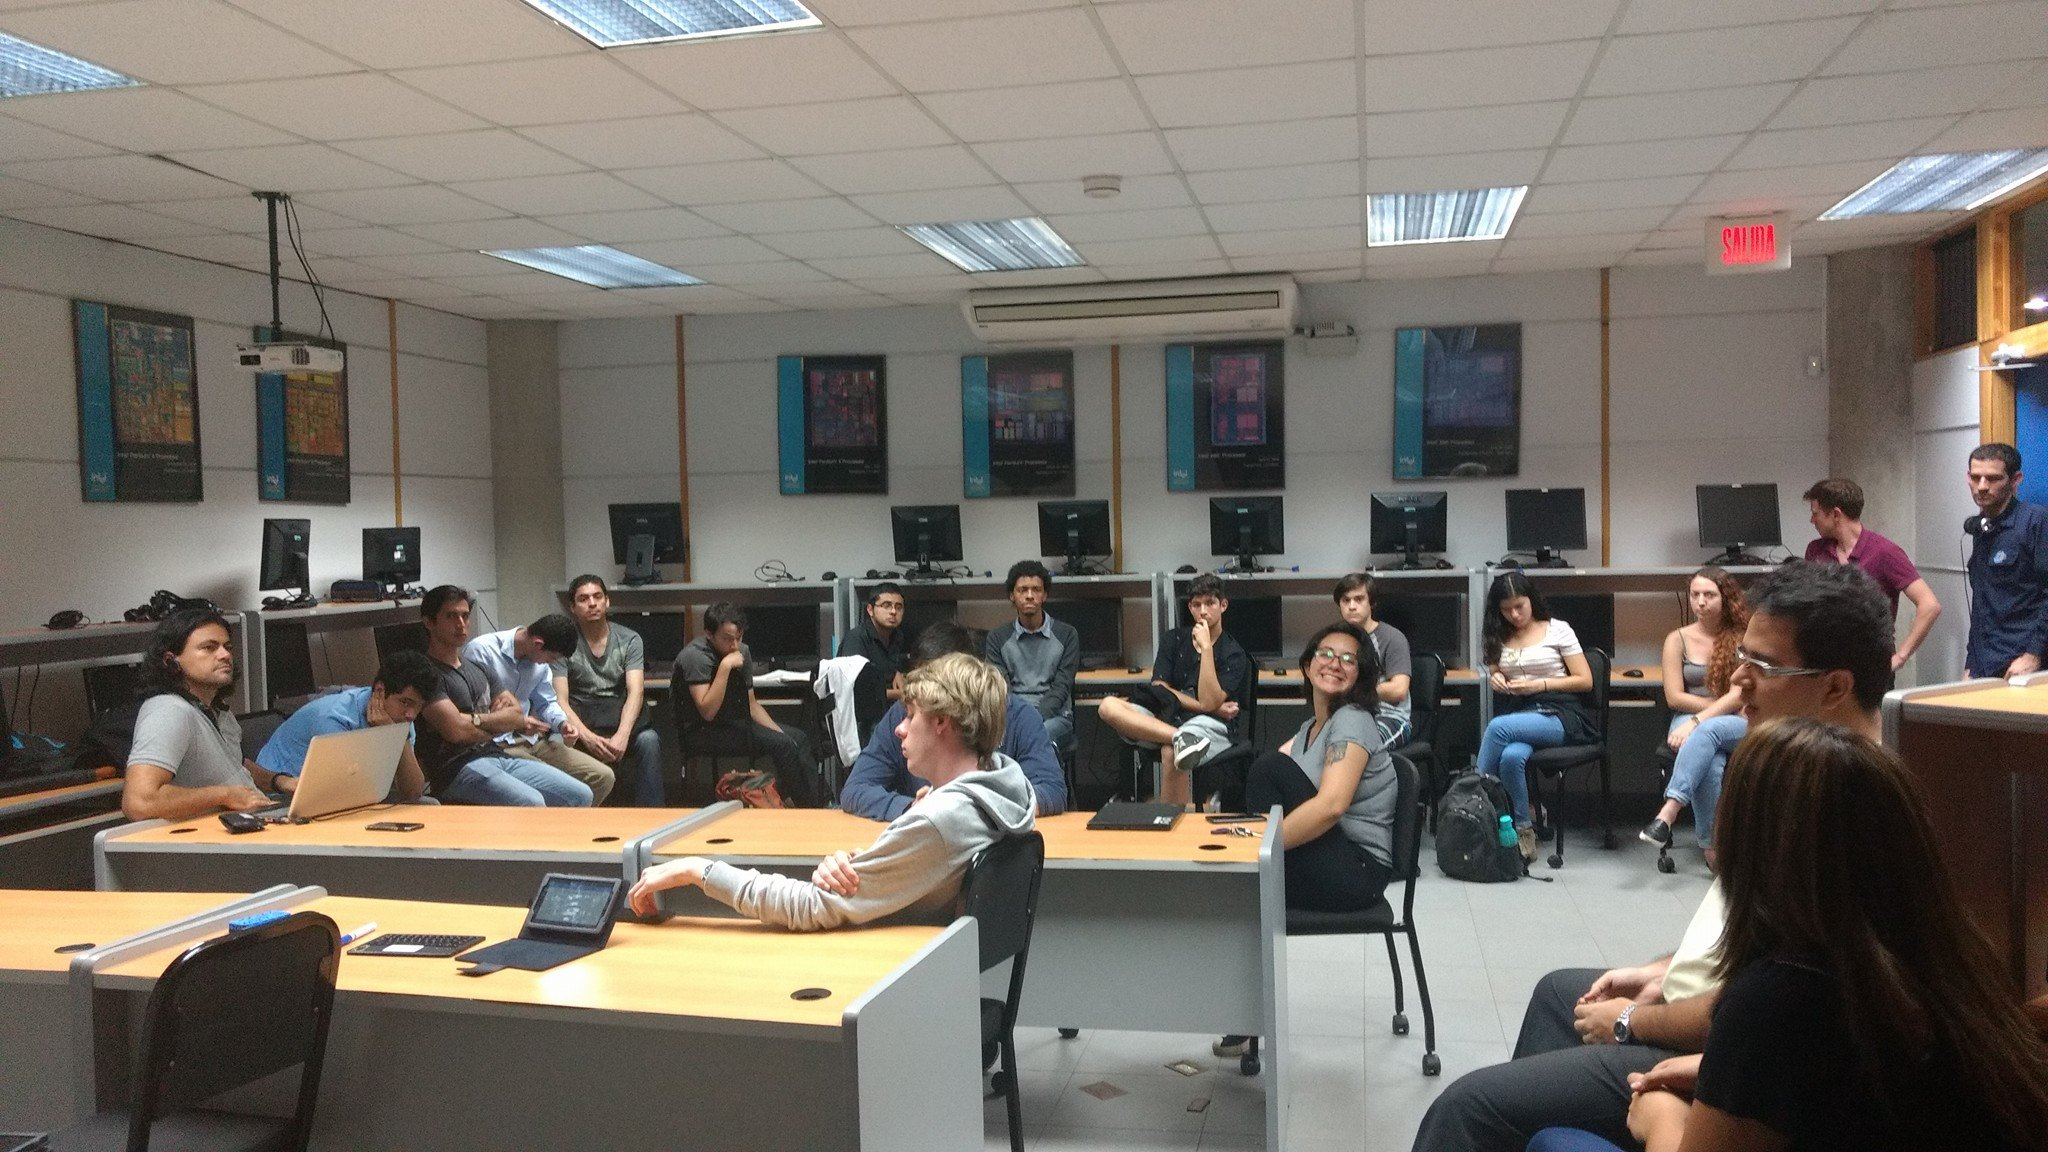
\includegraphics[width=1\textwidth]{img/integrantes.jpg}
       \end{figure}
    \end{center}
\end{frame}

\begin{frame}{Areas}
   \begin{itemize}
      \item Robótica de servicio
      \item Sistemas cognitivos
      \item Prototipado
   \end{itemize}
\end{frame}

\begin{frame}{Robot Humanoide}
  \begin{columns}
     \column{0.6\textwidth}
        \begin{itemize}
          \item Manipulación avanzada de objetos
          \item Percepción de su entorno
          \item Capacidades emocionales
          \item Colaboración humano - robot
          \item Tareas cotidianas
          	\begin{itemize}
          		\item Cocinar
                \item Organizar utensilios
          	\end{itemize}
          \item Tareas industriales
          	\begin{itemize}
          		\item Manufactura
                \item Despacho
          	\end{itemize}
         \end{itemize}
      \column{0.4\textwidth}
         \begin{center}
            \begin{figure}
               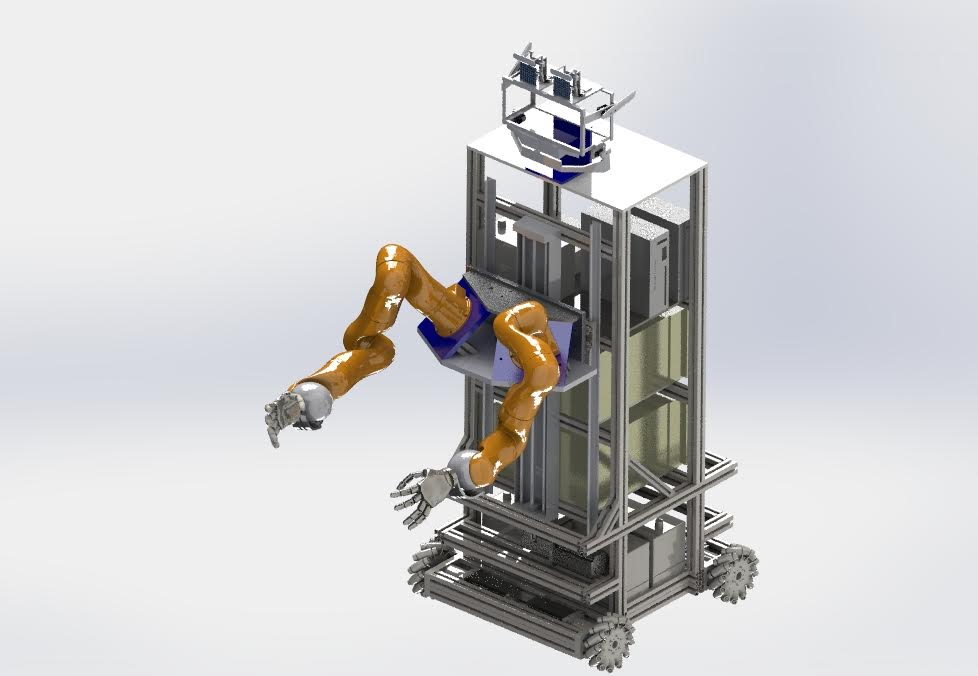
\includegraphics[width=1\textwidth]{img/robot.jpg}
            \end{figure}
         \end{center}
  \end{columns}
\end{frame}

\begin{frame}{Robot humanoide}
	\begin{center}
		\begin{figure}
			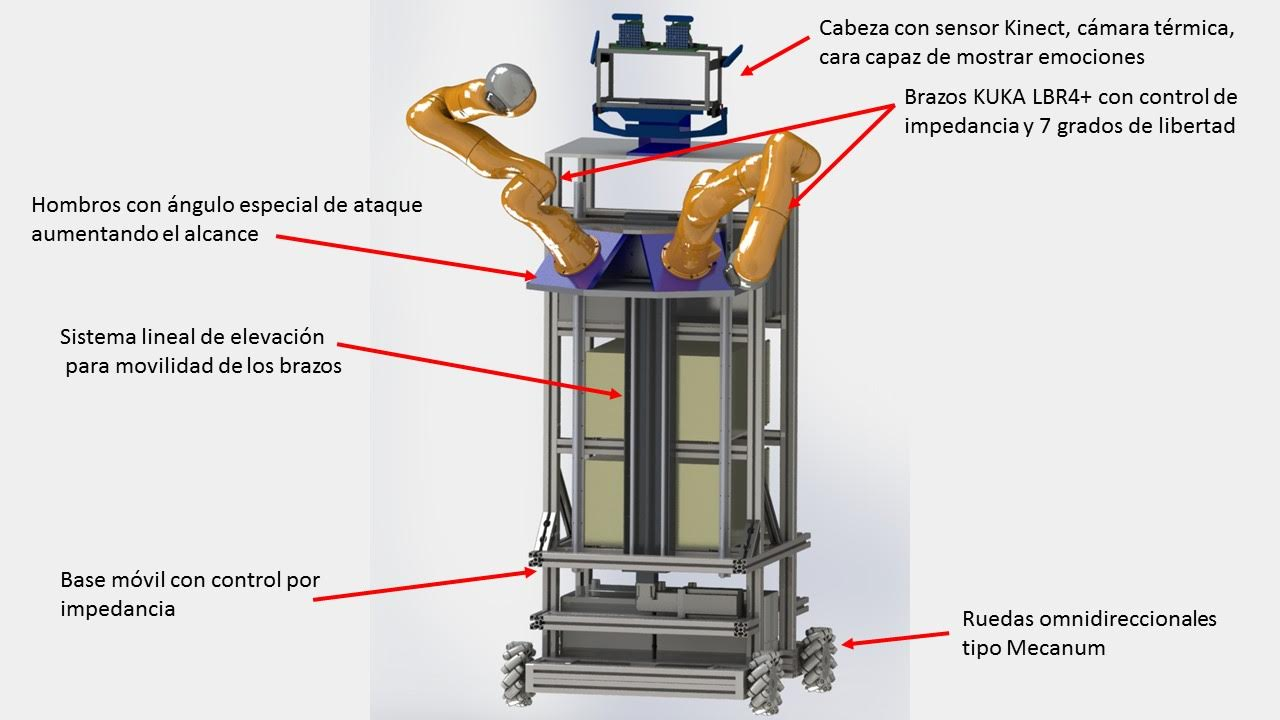
\includegraphics[width=1\textwidth]{img/robot-info.jpg}
		\end{figure}
	\end{center}
\end{frame}

\section{Microcontroladores}

\begin{frame}{¿Qué son microcontroladores?}
	\begin{itemize}
		\item "Computadora"
        	\begin{itemize}
        		\item Microprocesador
                \item Periféricos
        	\end{itemize}
        \item Recursos limitados
        \item Uso específico
	\end{itemize}
\end{frame}

\begin{frame}{Avance tecnológico}
	\begin{itemize}[<+- | alert@+>]
		\item 8 bits - Generador de reloj (8085)
        \item Memoria EPROM (8051)
        \item Flash, Amplio uso hobbytista (PIC's)
        \item Amplia comunicación, Popularización (AVR)
        \item 32 bits (JackRabbit, 80251, ARM)
        \item Popularización extrema (Arduino)
	\end{itemize}
\end{frame}

\begin{frame}{Usos}
	\begin{itemize}
		\item Automatización (Robótica)
        \item \textit{Wearables}
        \item Internet de las cosas
        \item Domótica
        \item \textit{Animatronics}
	\end{itemize}
\end{frame}

\begin{frame}{Tipos}
	\begin{columns}
    	\column{0.6\textwidth}
            \begin{itemize}
                \item Arduino - Genuino
                \item BeagleBone \alert{*}
                \item Raspberry Pi \alert{*}
                \item STM32
            \end{itemize}
        \column{0.4\textwidth}
			\begin{center}
				\begin{figure}
					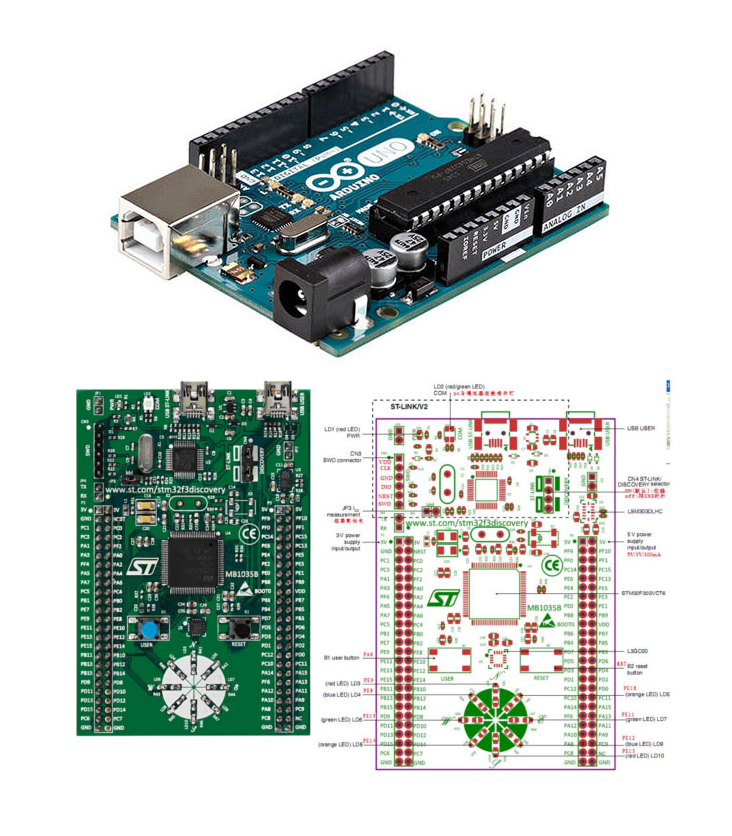
\includegraphics[width=1\textwidth]{img/micros.png}
				\end{figure}
			\end{center}
	\end{columns}
\end{frame}

\begin{frame}{STM32}
	\begin{columns}
    	\column{0.6\textwidth}
			\begin{itemize}
				\item 72 Mhz a 200 Mhz
                \item Multi-puerto (I2C, SPI, CANBUS, USB, UART)
                \item Alta densidad de almacenamiento (MBs)
                \item 200+ pines
                \item DMA, Interfaz LCD, Touchscreen
			\end{itemize}
        \column{0.4\textwidth}
			\begin{center}
				\begin{figure}
					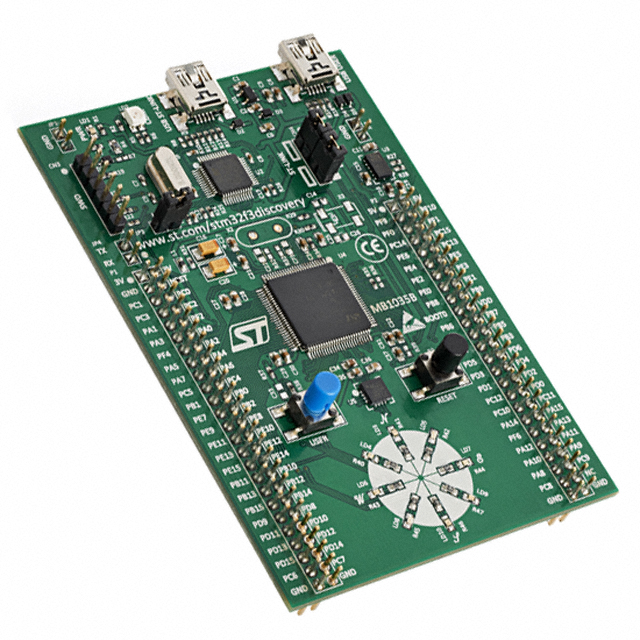
\includegraphics[width=1\textwidth]{img/f3discovery.jpg}
				\end{figure}
			\end{center}
	\end{columns}
\end{frame}

\begin{frame}{Raspberry Pi}
	\begin{columns}
    	\column{0.6\textwidth}
			\begin{itemize}
				\item Micro-computadora
                	\begin{itemize}
                		\item CPU 1GHz Quad-Core
                        \item 1GB RAM
                	\end{itemize}
                \item Linux
                \item 40 pines
                \item Múltiples librerías
			\end{itemize}
        \column{0.4\textwidth}
			\begin{center}
				\begin{figure}
					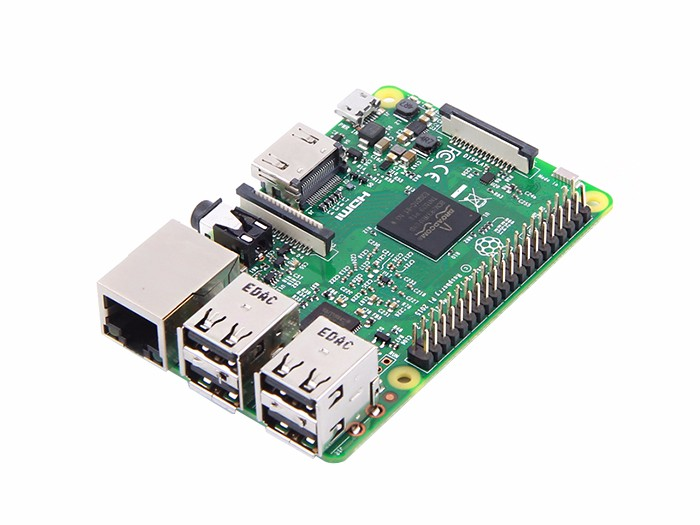
\includegraphics[width=1\textwidth]{img/pi3.jpg}
				\end{figure}
			\end{center}
	\end{columns}
\end{frame}

\section{LibOpenCM3}

\begin{frame}{¿Qué es?}
	\begin{itemize}
		\item Biblioteca de desarrollo
        \item Código abierto
        \item Microprocesadores ARM-Cortex M4
        \item Soporte a STM32, entre otros
	\end{itemize}
\end{frame}

\section{Proyectos}

\begin{frame}{Base Omnidireccional}
	\begin{columns}
    	\column{0.6\textwidth}
			\begin{itemize}
            	\item Desplazamiento
                	 \begin{itemize}
                	 	\item Todas direcciones 
                	 \end{itemize}
                \item Controlable
				\item Open-COROCO
                \item STM32F4 Discovery
                \item \href{https://www.facebook.com/ArcosLab/videos/vb.476608722370710/878271378871107/?type=2&theater}{Demo}
			\end{itemize}
        \column{0.4\textwidth}
			\begin{center}
				\begin{figure}
					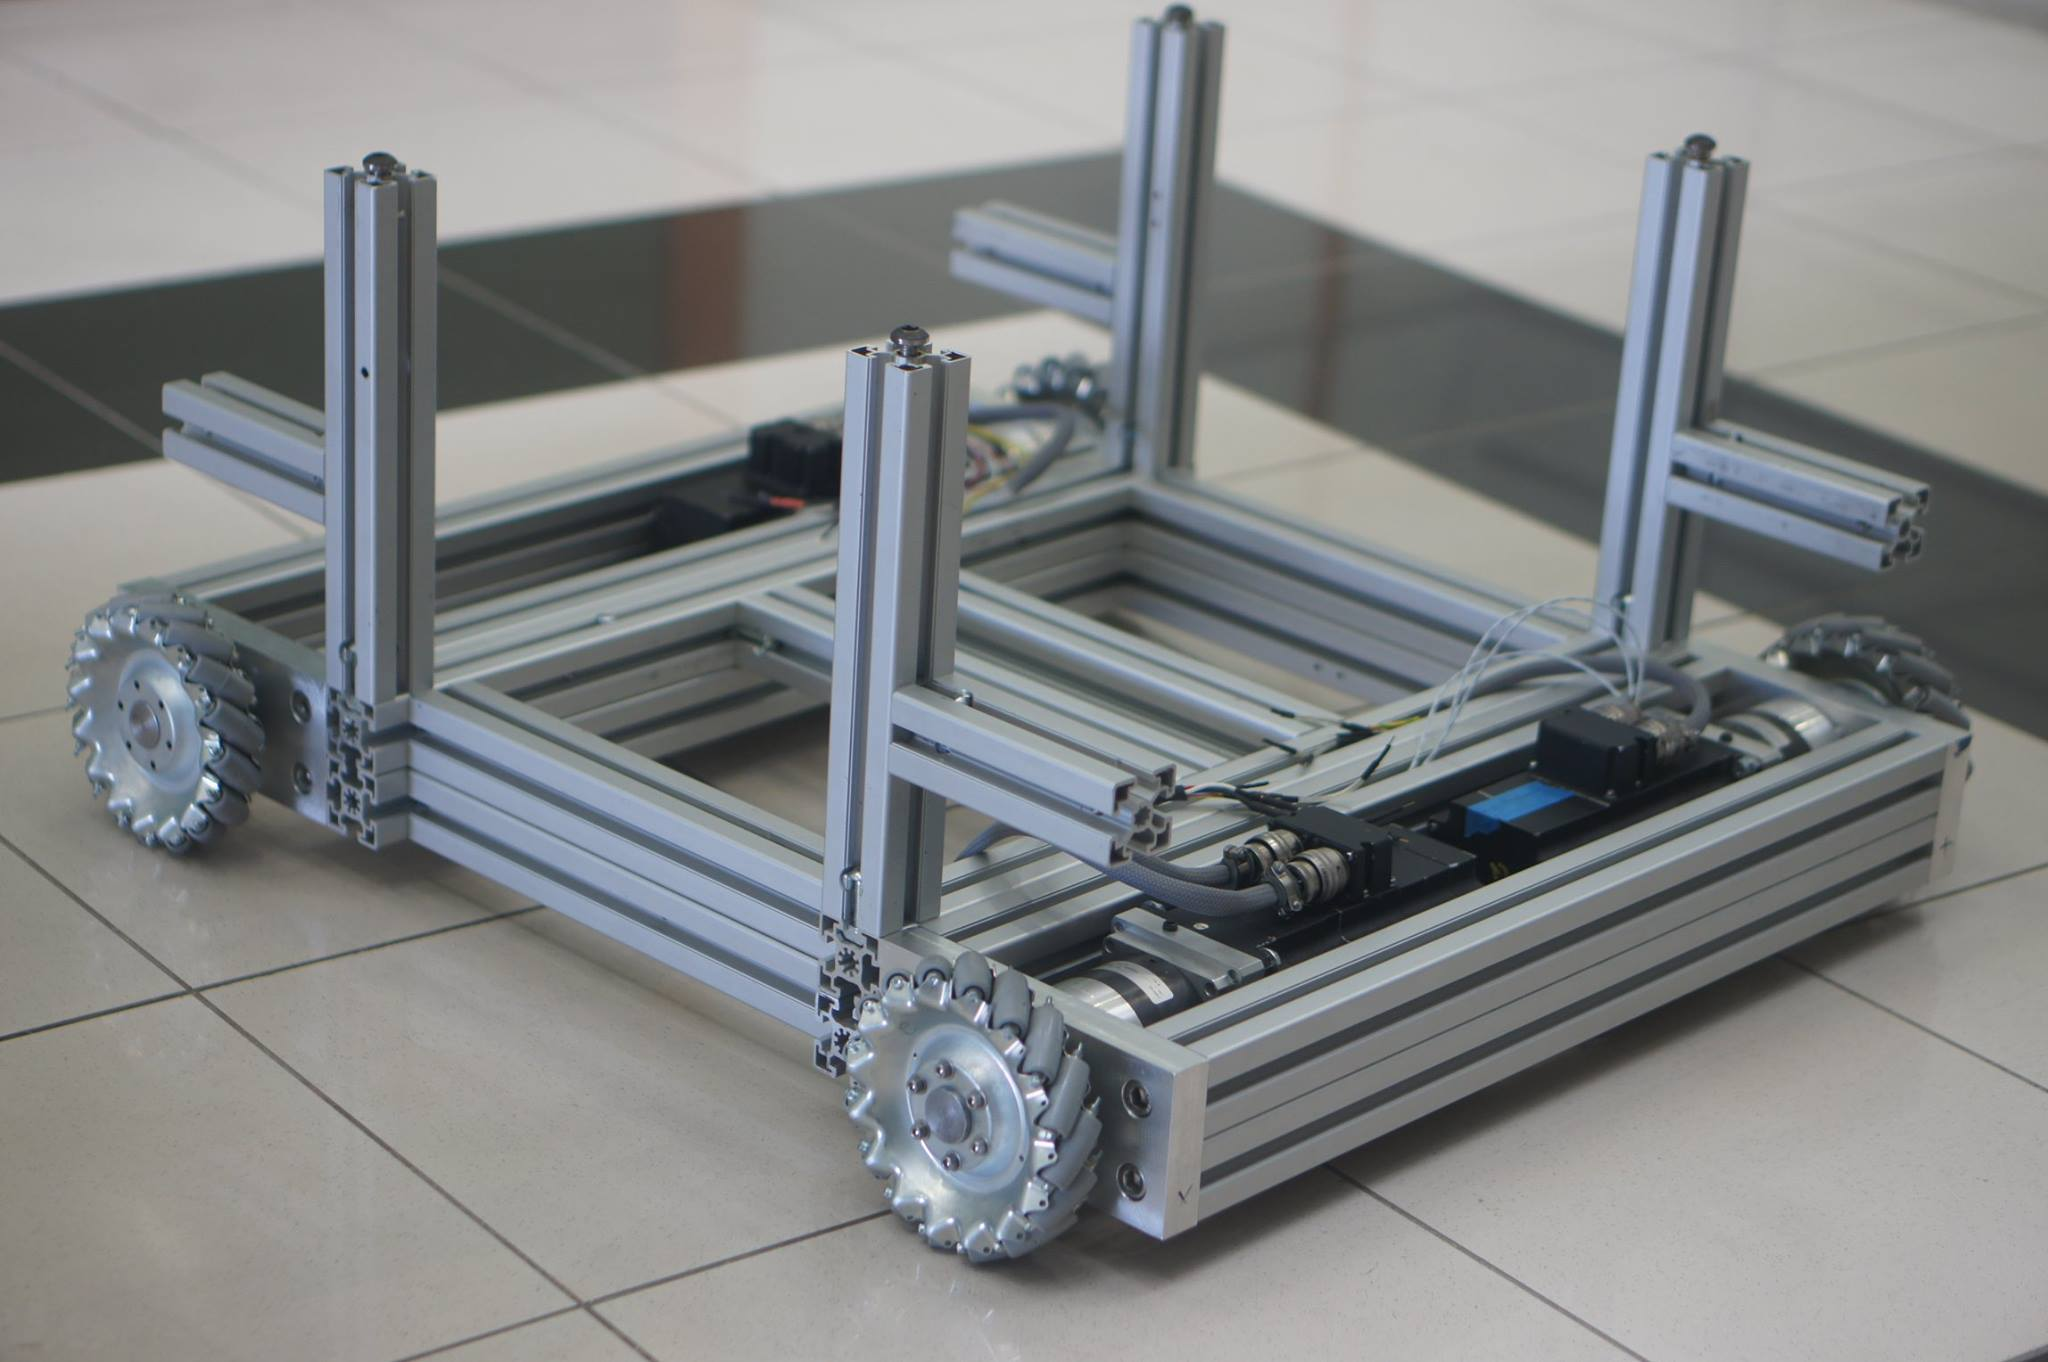
\includegraphics[width=1\textwidth]{img/base.jpg}
				\end{figure}
			\end{center}
	\end{columns}
\end{frame}

\begin{frame}{Open-COROCO}
	\begin{itemize}
		\item Open COmpliant RObot COntroller
        \item Articulación con \textit{control suave}
        \item STM32F4 Discovery
        \item \href{https://www.facebook.com/ArcosLab/videos/vb.476608722370710/814718461893066/?type=2&theater}{Demo}
	\end{itemize}
\end{frame}

\begin{frame}{Cuello}
	\begin{columns}
    	\column{0.6\textwidth}
			\begin{itemize}
            	\item Capacidad de percibir su entorno
                	\begin{itemize}
                		\item Movimiento vertical
                        \item Movimiento horizontal
                	\end{itemize}
                \item Control
                	\begin{itemize}
                		\item Velocidad
                        \item Posición
                	\end{itemize}
                \item Múltiples motores
                	\begin{itemize}
                		\item Control independiente
                	\end{itemize}
				\item STM32F4 Discovery
			\end{itemize}
        \column{0.4\textwidth}
			\begin{center}
				\begin{figure}
					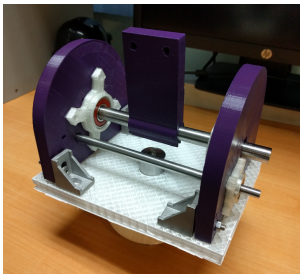
\includegraphics[width=1\textwidth]{img/cuello.png}
				\end{figure}
			\end{center}
	\end{columns}
\end{frame}

\begin{frame}{Cara emocional}
	\begin{columns}
    	\column{0.6\textwidth}
			\begin{itemize}
            	\item Expresar emociones
                	\begin{itemize}
                    	\item Confortable
                		\item Sorprendido
                        \item Triste
                        \item Feliz
                	\end{itemize}
                \item Comunicación con personas
				\item Arduino -> Raspberry-Pi 
			\end{itemize}
        \column{0.4\textwidth}
			\begin{center}
				\begin{figure}
					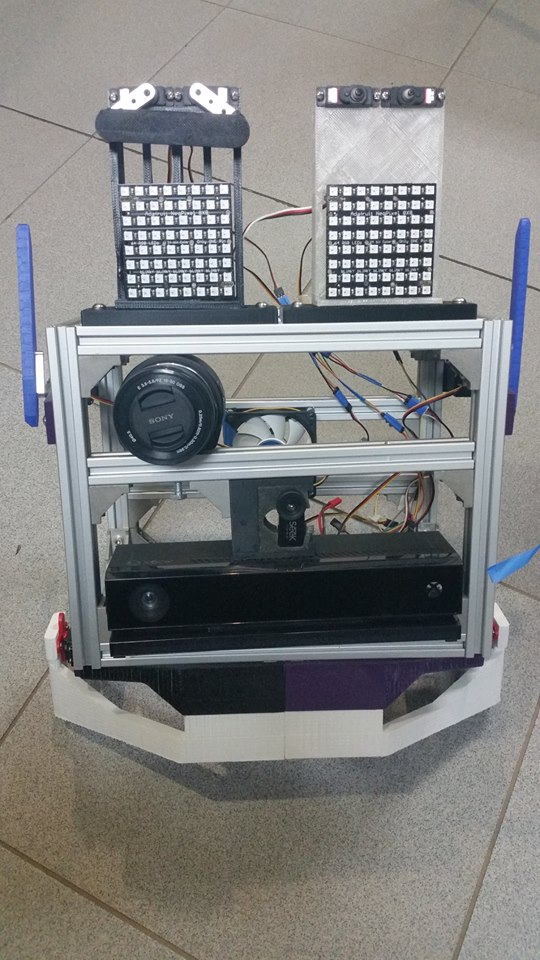
\includegraphics[width=1\textwidth]{img/cara.jpg}
				\end{figure}
			\end{center}
	\end{columns}
\end{frame}

\section{Microcontroladores vs Sistemas embebidos}

\begin{frame}{Comparativa}
	\begin{itemize}
		\item Tiempo real -> \alert{Microcontrolador}
        \item Alto procesamiento de datos -> \alert{Sistemas embebidos}
        \item Precio
        \item Consumo de energía -> \alert{Microcontrolador}
        \item Conectividad de red -> \alert{Sistema embebidos}
        \item Facilidad de desarrollo -> \alert{Sistema embebidos}
        \item Librerías disponibles -> \alert{Sistema embebidos}
        \item Tamaño -> \alert{Microcontrolador}
        \item Desarrollo personalizado -> \alert{Microcontrolador}
	\end{itemize}
\end{frame}

\section{Conclusiones}

\begin{frame}{Sumario}
   \begin{itemize}
      \item ARCOS-Lab
         \begin{itemize}
            \item Entorno
            \item Proyectos
            \item Robot Humanoide
         \end{itemize}
      \item Microcontroladores
      \item LibOpenCM3
      \item Proyectos
         \begin{itemize}
            \item Base Omnidireccional
            \item Open-COROCO
            \item Cuello
            \item Cara emocional
         \end{itemize}
      \item Microcontroladores vs Sistemas embebidos 
   \end{itemize}
\end{frame}

\begin{frame}[standout]
  ¿Preguntas?
\end{frame}

\begin{frame}[standout]
  ¡Muchas gracias!
\end{frame}

\begin{comment}
\section{Elements}

\begin{frame}[fragile]{Typography}
      \begin{verbatim}The theme provides sensible defaults to
\emph{emphasize} text, \alert{accent} parts
or show \textbf{bold} results.\end{verbatim}

  \begin{center}becomes\end{center}

  The theme provides sensible defaults to \emph{emphasize} text,
  \alert{accent} parts or show \textbf{bold} results.
\end{frame}

\begin{frame}{Font feature test}
  \begin{itemize}
    \item Regular
    \item \textit{Italic}
    \item \textsc{SmallCaps}
    \item \textbf{Bold}
    \item \textbf{\textit{Bold Italic}}
    \item \textbf{\textsc{Bold SmallCaps}}
    \item \texttt{Monospace}
    \item \texttt{\textit{Monospace Italic}}
    \item \texttt{\textbf{Monospace Bold}}
    \item \texttt{\textbf{\textit{Monospace Bold Italic}}}
  \end{itemize}
\end{frame}

\begin{frame}{Lists}
  \begin{columns}[T,onlytextwidth]
    \column{0.33\textwidth}
      Items
      \begin{itemize}
        \item Milk \item Eggs \item Potatos
      \end{itemize}

    \column{0.33\textwidth}
      Enumerations
      \begin{enumerate}
        \item First, \item Second and \item Last.
      \end{enumerate}

    \column{0.33\textwidth}
      Descriptions
      \begin{description}
        \item[PowerPoint] Meeh. \item[Beamer] Yeeeha.
      \end{description}
  \end{columns}
\end{frame}

\begin{frame}{Animation}
  \begin{itemize}[<+- | alert@+>]
    \item \alert<4>{This is\only<4>{ really} important}
    \item Now this
    \item And now this
  \end{itemize}
\end{frame}

\begin{frame}{Quotes}
  \begin{quote}
    Veni, Vidi, Vici
  \end{quote}
\end{frame}

\begin{frame}{References}
  Some references to showcase [allowframebreaks] \cite{knuth92,ConcreteMath,Simpson,Er01,greenwade93}
\end{frame}

\begin{frame}[allowframebreaks]{References}

  \bibliography{demo}
  \bibliographystyle{abbrv}

\end{frame}

\begin{frame}[standout]
  ¿Preguntas?
\end{frame}
\end{comment}

\end{document}